\documentclass[12pt]{article}
\usepackage{graphicx} % Required for inserting images
\usepackage{hyperref}
\usepackage{makecell}
\usepackage{makeidx}
\usepackage{eurosym}
\usepackage{amsmath}
\usepackage{fancyhdr}
\newcommand{\firstPage}{
    \thispagestyle{empty}
    \begin{figure}
    \centering
    
\includegraphics[scale=0.7]{Swellfish_logo.png}
    \end{figure}
    \author{
        \date{}
        \href{mailto://swellfish14@gmail.com}{swellfish14@gmail.com} \\
    } 
}
\usepackage{hyperref}
\usepackage{array}
\usepackage{tabularx}
\usepackage{adjustbox}

\newcounter{verscount}
\setcounter{verscount}{0}
\newcommand{\addversione}[5]{
	\ifdefined\setversione
		\setversione{#1}
	\else\fi
	\stepcounter{verscount}
	\expandafter\newcommand%
		\csname ver\theverscount \endcsname{#1&#2&#3&#4&#5}
}

\newcommand{\listversioni}{
	\ifnum\value{verscount}>1
		\csname ver\theverscount \endcsname
		\addtocounter{verscount}{-1}
		\\\hline
		\listversioni
	\else
		\csname ver\theverscount \endcsname\\\hline
	\fi
}

\newcommand{\makeversioni}{
	\begin{center}
		\begin{tabularx}{\textwidth}{|c|c|X|X|X|}
		\hline
		\textbf{Versione} & \textbf{Data} & \textbf{Redattore} & \textbf{Verificatore} & \textbf{Descrizione} \\
		\hline
		\listversioni
		\end{tabularx}
	\end{center}
	\clearpage
}

\fancypagestyle{genericDocstyle}{
	\pagestyle{fancy}
	\lhead{
\includegraphics[width=1cm]{Swellfish_logo.png}}
	\rhead{Norme di progetto}
}

%\hypersetup{colorlinks=true,urlcolor=blue}

%\newcommand{\tableContent}{

	%{
		%\hypersetup{linkcolor=black}
		%\tableofcontents
	%}
%}
\begin{document}

\graphicspath{ {../templates/img/} {./img}}

\title{Piano di progetto}

\firstPage

\sethdr{Piano di qualifica}


\maketitle

\begin{center}
	\begin{tabular}{r | l}
		\multicolumn{2}{c}{\textit{Informazioni}}                         \\
		\hline

		\textit{Redattori}    &
		[Davide Porporati, Elena Marchioro, Francesco Naletto]\makecell{} \\

		\textit{Revisori}     &
		[Jude Vensil Braceros]\makecell{}                                 \\
		\textit{Responsabili} &
		[Andrea Veronese]\makecell{}                                      \\
		\textit{Uso}          &
		[Esterno]\makecell{}                                              \\
	\end{tabular}
\end{center}

\begin{center}
	\textbf{Descrizione}\\
	File contenente il piano di qualifica. Contiene le metriche e i criteri di accettazione dei prodotti.
\end{center}

\pagebreak

\tableofcontents
\pagebreak

\printindex

\addversione{0.0.1}{25/04/2023}{Andrea Veronese}{Davide Porporati}{Creata struttura di base del documento}
\addversione{0.0.2}{27/04/2023}{Davide Porporati, Elena Marchioro, Francesco Naletto}{Jude Vensil Braceros}{Modificata la struttura del documento}
\makeversioni

\section{Introduzione}
\subsection{Scopo del documento}
Questo documento ha lo scopo di definire le strategia di validazione e verifica addottate per garantire la qualità del prodotto.
Per raggiungere questo obbiettivo viene applicato un sistema di verifica continua sui processi e sulle attività del gruppo, questo permette di ottenere un miglioramento continuo.
Il documento viene redatto in maniera incrementale, ovvero viene tenuto in costante aggiornamento durante tutta la durata del progetto.
\subsection{Scopo del capitolato}
In Italia, il prezzo del gas è aumentato significativamente, e il consumo di gas e carbone sta portando ad un aumento delle emissioni di gas serra e CO2. Per affrontare il problema del costo dell'energia, molti comuni stanno tagliando l'illuminazione pubblica, ma questo può essere evitato attraverso l'implementazione di un sistema di illuminazione pubblica ottimizzato, che consentirebbe sia la sicurezza stradale che il risparmio energetico ed economico.
Nel capitolato in questione si vuole implementare questa soluzione tramite un applicativo web. Quest'ultimo permetterebbe la gestione dell'illuminazione in modo sia automatico che manuale.
\section{Qualità di processo}

\subsection{Processi primari}

\subsubsection{Fornitura}
\textbf{Metriche:}
\begin{itemize}
	\item MPC01: Actual Cost (AV)
	      \begin{itemize}
		      \item \textbf{Calcolo della metrica}: Somma dei costi tracciati dal gruppo
		      \item \textbf{Valore ottimale}: $\le BAC$
		      \item \textbf{Valore accettabile}: $\le BAC$
	      \end{itemize}
	\item MPC02: Planned Value (PV)
	      \begin{itemize}
		      \item \textbf{Calcolo della metrica}: Percentuale di completamento del progetto pianificata * BAC
		      \item \textbf{Valore ottimale}: $\le BAC$
		      \item \textbf{Valore accettabile}: $\le BAC$
	      \end{itemize}
	\item MPC03: Earned Value (EV)
	      \begin{itemize}
		      \item \textbf{Calcolo della metrica}: Percentuale dell'effettivo stato di completamento del progetto * BAC
		      \item \textbf{Valore ottimale}: $\ge 0$
		      \item \textbf{Valore accettabile}: $\le BAC$
	      \end{itemize}
	\item MPC04: Cost Variance (CV)
	      \begin{itemize}
		      \item \textbf{Calcolo della metrica}:  EV - AC
		      \item \textbf{Valore ottimale}: $\ge 0\%$
		      \item \textbf{Valore accettabile}: $\ge -10\%$
	      \end{itemize}
	\item MPC05: Schedule Variance (SV)
	      \begin{itemize}
		      \item \textbf{Calcolo della metrica}:  EV - PV
		      \item \textbf{Valore ottimale}: $\ge 0\%$
		      \item \textbf{Valore accettabile}: $\ge -10\%$
	      \end{itemize}

	\item MPC06: Cost Performance Index (CPI)
			\begin{itemize}
				\item \textbf{Calcolo della metrica}:  EV / AC
				\item \textbf{Valore ottimale}: $\ge 1$
				\item \textbf{Valore accettabile}: $\ge 0,9$
			\end{itemize}
	
	\item MPC07: Estimated At Completition (EAC)
	      \begin{itemize}
		      \item \textbf{Calcolo della metrica}:  BAC / CPI
		      \item \textbf{Valore ottimale}: = BAC
		      \item \textbf{Valore accettabile}: $\ge BAC - 3\% ; \le BAC + 3\% $
	      \end{itemize}
	\item MPC08: Estimate To Completition (ETC)
	      \begin{itemize}
		      \item \textbf{Calcolo della metrica}:  (BAC - EV) / CPI
		      \item \textbf{Valore ottimale}: $\ge 0\%$
		      \item \textbf{Valore accettabile}: $\le EAC$
	      \end{itemize}
\end{itemize}

\subsection{Processi di supporto}
\subsubsection{Documentazione}
\textbf{Metriche:}
\begin{itemize}
	\item MPC09: Indice di Gulpease
	      \begin{itemize}
		      \item \textbf{Calcolo della metrica}:  89 + $\frac{300*(F) - 10 * (L)}{(P)}$
		            \begin{itemize}
			            \item \textbf{L} = Numero di lettere nel testo
			            \item \textbf{P} = Numero di parole nel testo
			            \item \textbf{F} = Numero di frasi nel testo
		            \end{itemize}
		      \item \textbf{Valore ottimale}: 100 \%
		      \item \textbf{Valore accettabile}: $\ge 60\%$
	      \end{itemize}
\end{itemize}
\begin{itemize}
	\item MPC10: Errori ortografici
	      \begin{itemize}
		      \item \textbf{Calcolo della metrica}: numero errori ortografici presenti nel testo
		      \item \textbf{Valore ottimale}: 0
		      \item \textbf{Valore accettabile}: 0
	      \end{itemize}
\end{itemize}

\subsubsection{Verifica}

\textbf{Metriche:}
\begin{itemize}
	\item MPC11: Code Coverage
	      \begin{itemize}
		      \item \textbf{Calcolo della metrica}:  (Numero di righe di codice testate / Numero totale di righe di codice) * 100
		      \item \textbf{Valore ottimale}: 100\%
		      \item \textbf{Valore accettabile}: 80\%
	      \end{itemize}
\end{itemize}

\subsection{Processi organizzativi}

\section{Qualità di prodotto}
\subsection{Introduzione}
Per assicurare la qualità del prodotto, abbiamo adottato lo standard ISO/IEC 9126 come punto di riferimento. In questa sezione, forniamo i valori ottimali e accettabili per le metriche selezionate dal gruppo SWEllFish.



\subsection{Affidabilità}
	Indica la capacità del prodotto di svolgere le sue funzioni, anche in presenza di errori, provando ad eliminarne la loro incidenza.
	\\\\
	\textbf{Metriche}:
	\begin{itemize}
		\item MPD01: Percentuale di difetti del prodotto.
		\begin{itemize}	
			\item Valore ottimale: 80\%.
			\item Valore accettabile: 60\%.
			\item Note: I valori possono essere modificati.
		\end{itemize}
	\end{itemize}


\subsection{Efficienza}
	Indica la capacità del prodotto di svolgere le sue funzioni utilizzando il minor numero di risorse possibile.
	\\\\
	\textbf{Metriche}:
	\begin{itemize}
		\item MPD02: Tempo medio di risposta.
		\begin{itemize}	
			\item Metrica di misurazione: Secondi.
			\item Valore ottimale: 5 secondi.
			\item Valore accettabile: 7 secondi.
		\end{itemize}
	\end{itemize}

\subsection{Funzionalità}

	Indica la capacità del prodotto di svolgere tutte le funzioni previste in modo completo e corretto.
	\\\\
	\textbf{Metriche}:
	\begin{itemize}
		\item MPD03: Percentuale di copertura dei requisiti.
		\begin{itemize}	
			\item Valore ottimale: 100\% dei requisiti obbligatori e 80\% dei requisiti opzionali.
			\item Valore accettabile: 100\% dei requisiti obbligatori.
		\end{itemize}
	\end{itemize}

\subsection{Manutenibilità}
	Indica la capacità del prodotto di essere modificato e mantenuto in modo efficiente.
	\\\\
	\textbf{Metriche}:
		\begin{itemize}
			\item MPD04: Percentuale di comprensibilità del codice.
			\begin{itemize}	
				\item Valore ottimale: 85\% - 100\%.
				\item Valore accettabile: 65\%.
			\end{itemize}
		\end{itemize}

\subsection{Portabilità}
	Indica la capacità del prodotto di essere utilizzato in diverse piattaforme e ambienti.
	\\\\
	\textbf{Metriche}:
		  \begin{itemize}
			\item MPD05: Percentuale di compatibilità del prodotto.
			\begin{itemize}	
				\item Valore ottimale: 85\% - 100\%.
				\item Valore accettabile: 60\%.
			\end{itemize}
		\end{itemize}


\subsection{Usabilità}
	Indica la capacità del prodotto di essere utilizzato in modo efficace, efficiente e soddisfacente dagli utenti finali.
	\\\\
	\textbf{Metriche:}
		  \begin{itemize}
			\item MPD06: Numero di errori compiuti dagli utenti durante l'utilizzo del prodotto.
			\begin{itemize}	
				\item Valore ottimale: Inferiore a 1 errore per utente.
				\item Valore accettabile: Inferiore a 2 errori per utente.
			\end{itemize}
		\end{itemize}
		  


\section{Specifica di test}
\section {Resoconto attività di verifica}
\subsection{Planning Value, Actual Cost e Earned Value}
\begin{center}
	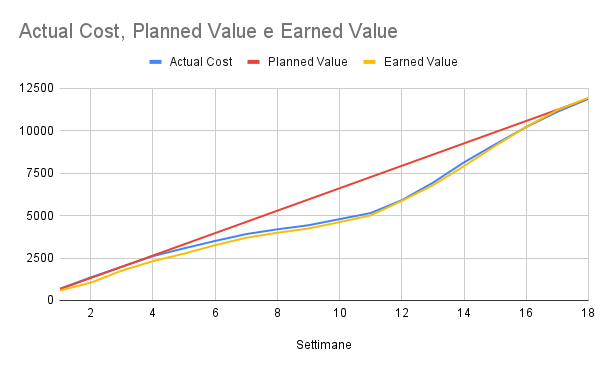
\includegraphics[scale=0.5]{AC_PV_EV.png}
\end{center}
\subsection{Cost Variance e Schedule Variance}
\begin{center}
	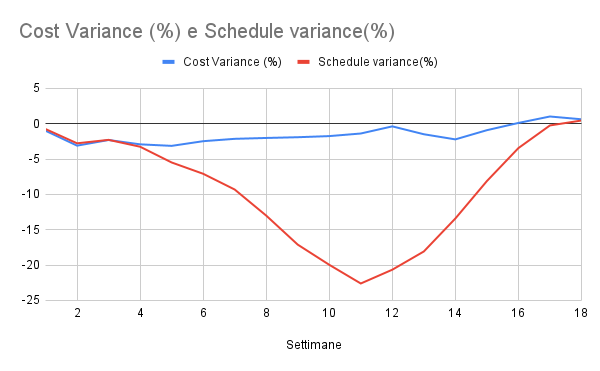
\includegraphics[scale=0.5]{Cost_Variance_Schedule_Variance.png}
\end{center}

\subsection{Eastimate at completition e Estimate to Complete}
\begin{center}
	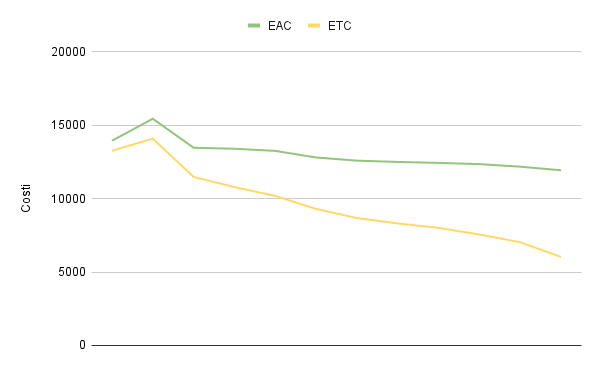
\includegraphics[scale=0.6]{EAC_ETC.png}
\end{center}
\subsection{Cost Performance Index}
\begin{center}
	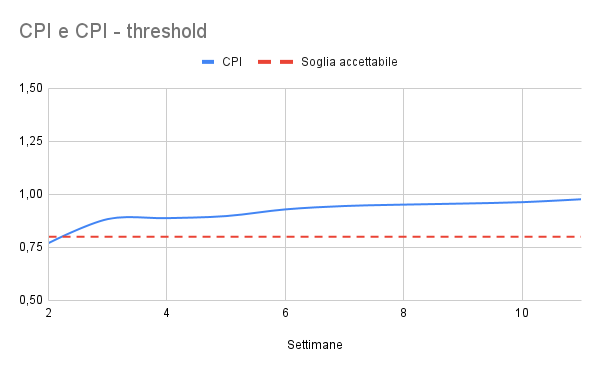
\includegraphics[scale=0.6]{CPI.png}
\end{center}


\end{document}
